\documentclass[letterpaper]{article}
\usepackage{geometry}
\usepackage{xcolor}
\usepackage{graphicx}
\usepackage{amsmath}
\usepackage[some]{background}
\usepackage{lipsum}

\definecolor{titlepagecolor}{cmyk}{1,.60,0,.40}

\DeclareFixedFont{\bigsf}{T1}{phv}{b}{n}{1.5cm}

\backgroundsetup{
scale=1,
angle=0,
opacity=1,
contents={\begin{tikzpicture}[remember picture,overlay]
 \path [fill=titlepagecolor] (-0.5\paperwidth,5) rectangle (0.5\paperwidth,10);  
\end{tikzpicture}}
}
\makeatletter                       
\def\printauthor{%                  
    {\large \@author}}              
\makeatother
\author{%
    Halse, Douglas \\
    Karlsson, Mattias \\
    Larsson, Johan \\
    Persson, Hannes \\
    Östmo, Marcus \\
    }
\begin{document}
\begin{titlepage}
\BgThispage
\newgeometry{left=1cm,right=4cm}
\vspace*{2cm}
\noindent
\textcolor{white}{\bigsf Sight tracking in Unity}
\vspace*{2.5cm}\par
\noindent
\begin{minipage}{0.35\linewidth}
    \begin{flushright}
        \printauthor
    \end{flushright}
\end{minipage} \hspace{15pt}
%
\begin{minipage}{0.02\linewidth}
    \rule{1pt}{175pt}
\end{minipage} \hspace{-10pt}
%
\begin{minipage}{0.6\linewidth}
\vspace{-2in}
    %\begin{abstract}
    %\end{abstract}
\end{minipage}
\end{titlepage}
\restoregeometry
\tableofcontents
\newpage
\section{Introduction}
This software is developed to help study different behaviors in human-computer interaction. It keeps track of where the user looks, for how long and where the user is located in 3D space. All of this information is saved to disk with timestamps in CSV-files. The software is designed to be easily implemented to any Unity project, by only having to add one script to the Camera in Unity. The information from the files makes it possible to replay a sequence based on the data.
The files contain the following information:\\
\begin{itemize}
\item Which game objects the user have looked at, and for how long in total.\\
\item A list sorted by time of which objects the user have been looking at, for how long and where the user was located when looking at the particular object.
\end{itemize}
\newpage
\section{Before first use - IMPORTANT!}
\subsection{Faulty data}
Do not start and stop the Sighttracker during the runtime of the scene, this forces the tracker to initialize and adds incorrect data to the CSV file. If you observe a “Starting...” in your CSV file, you have encountered this issue. If this issue has occurred, you have to manually exclude the starting time from further calculations based on the data or rerun the test again.
\subsection{Unique object names}
Do not name the unity gameobjects identically, the SightTracker package differentiates objects based on name. If you have two objects of the same name, when looking at either of them the stopwatch would run continually as if it were one object. This error is hard to notice in the CSV file unless you pay careful attention when running the test.
\subsection{Objects that block player view}
The SightTracker has not been extensively tested, there might be issues with using the tracker along with a complex playermodel. The SightTracker shoots out a beam and records the object that is hit, and certain playermodels might be in the way of the beam. If this is the case, it might be helpful to move the camera to a slightly different position in the playermodel.
\subsection{Unity Keycodes to specify keybinds}
You must use Unity keycodes when selecting keybindings for the debug HUD, keycodes can be found on Unity's website \cite{unitykeycode}.
\subsection{More than one scene}
The SightTracker package has only been tested while using a single scene. When running a program that changes scenes there will be undefined behaviour, this is not recommended.
\newpage
\section{Manual}
\subsection{Installation}
\begin{itemize}
\item \textbf{Importing to Unity}\\
1. Open up your project, go to 'Assets' in the top menu bar.\\[0.15in]
2. In the drop-down menu select 'Import package' and then 'Custom package'.
\begin{figure}[h!]
  \centering 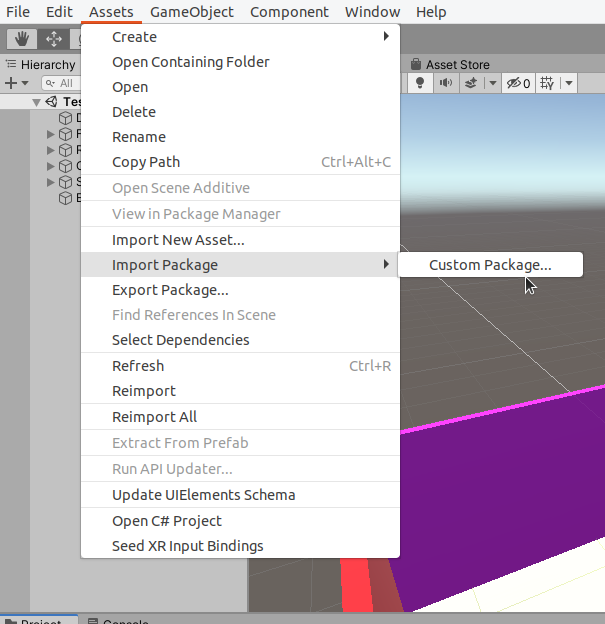
\includegraphics[keepaspectratio,scale=0.8]{ImportPackage.png}
  \caption{Importing a package in unity}
  \label{fig:unityimport}
\end{figure}
\\3. Locate the SightTracker package and select it.\\[0.15in]
4. You should now see the SightTracker folder in your project, open the folder and drag the script named SightTracker to the camera.\\
\item \textbf{Settings}\\
\begin{figure}[h!]
  \centering 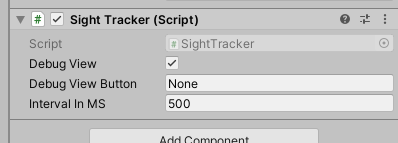
\includegraphics[keepaspectratio,scale=0.9]{SightTracker.png}
  \caption{SightTracker has been added to the camera}
  \label{fig:loadedtocamera}
\end{figure}

5. The figure above is what the Inspector of the camera should look like. From here you can choose a key to toggle the debug HUD of the SightTracker. The key must, however, be a Unity Keycode \cite{unitykeycode}. From here you can also select the sampling rate. The options are: Full, Half and Quarter. This means that the Sight Tracker either captures each frame, every other frame or every fourth frame.\\[0.15in]
6. The SightTracker will generate three different CSV-files on each run of the program, with timestamps to help distinguish each usage.
\end{itemize}
\subsubsection{CSV output}
The SightTracker package generates three different CSV files as mentioned earlier\\
\begin{itemize}
\item \textbf{CSVSequential} [Object, time]\\
Contains a list of which objects the user have been looking at in order and a duration for how long the object was looked at.
\item \textbf{CSVSummary} [Object, time]\\
Contains a summary of all objects looked at and the total time looked at each object.
\item \textbf{CSVTimeData} [3D Vector, 3D Vector, TimeStamp]\\
Contains two vectors, the first vector is where the player is looking, the second is the location of the user and the third is the time from start that the user is at this position and looks this direction.
\end{itemize}
\pagebreak
\subsection{Using SightTracker}
As long as the script was loaded properly onto your own Unity project and attached, as a script, to the camera it should automatically generate the aforementioned CSV files.\\
The output of the script is to the folder \texttt{'/path\_to\_your\_project/Sight\_tracker/'}.\\
The Record Rate setting is essentially the polling rate of the program. How often it records the users position and the direction of the camera. By setting this to \texttt{'Full'} the program records \textbf{every} frame which generates a huge CSV file if program runs for an extended period of time.\\[0.15in]
\texttt{'Full'} - Records the camera direction and position of every frame.\\
\texttt{'Half'} - Records the camera direction and position of every other frame.\\
\texttt{'Quarter'} - Records the camera direction and position every fourth frame.
\section{Graphical representation of data}
Since this software records a lot of data of what the user is looking at it would be nice to have a way to display the results. This could for example be using a pie or bar chart to show how long each object in the scene have been looked at by the user. Another way to display the collected data could be done by making a 3D heatmap over the entire scene.\\[0.15in]
As could be imagined, there are a lot of ways to display the data visually, and different users would most likely want it displayed in different ways.\\[0.15in]
Thus, we decided not to create an explicit program to display the data. Instead we are going to share some good resources for visualizing a csv file.\\[0.15in]
If the user wants to create some diagrams for the data, the library bokeh \cite{bokeh} is a great option. This library can create interactive visualization graphs for web browsers. And would a minimum amount of python code you could make this following bar chart with the generated csv data file. This chart can be viewed in any web browser and have features such as move, zoom and save.
\newpage
\begin{figure}[h!]
  \centering 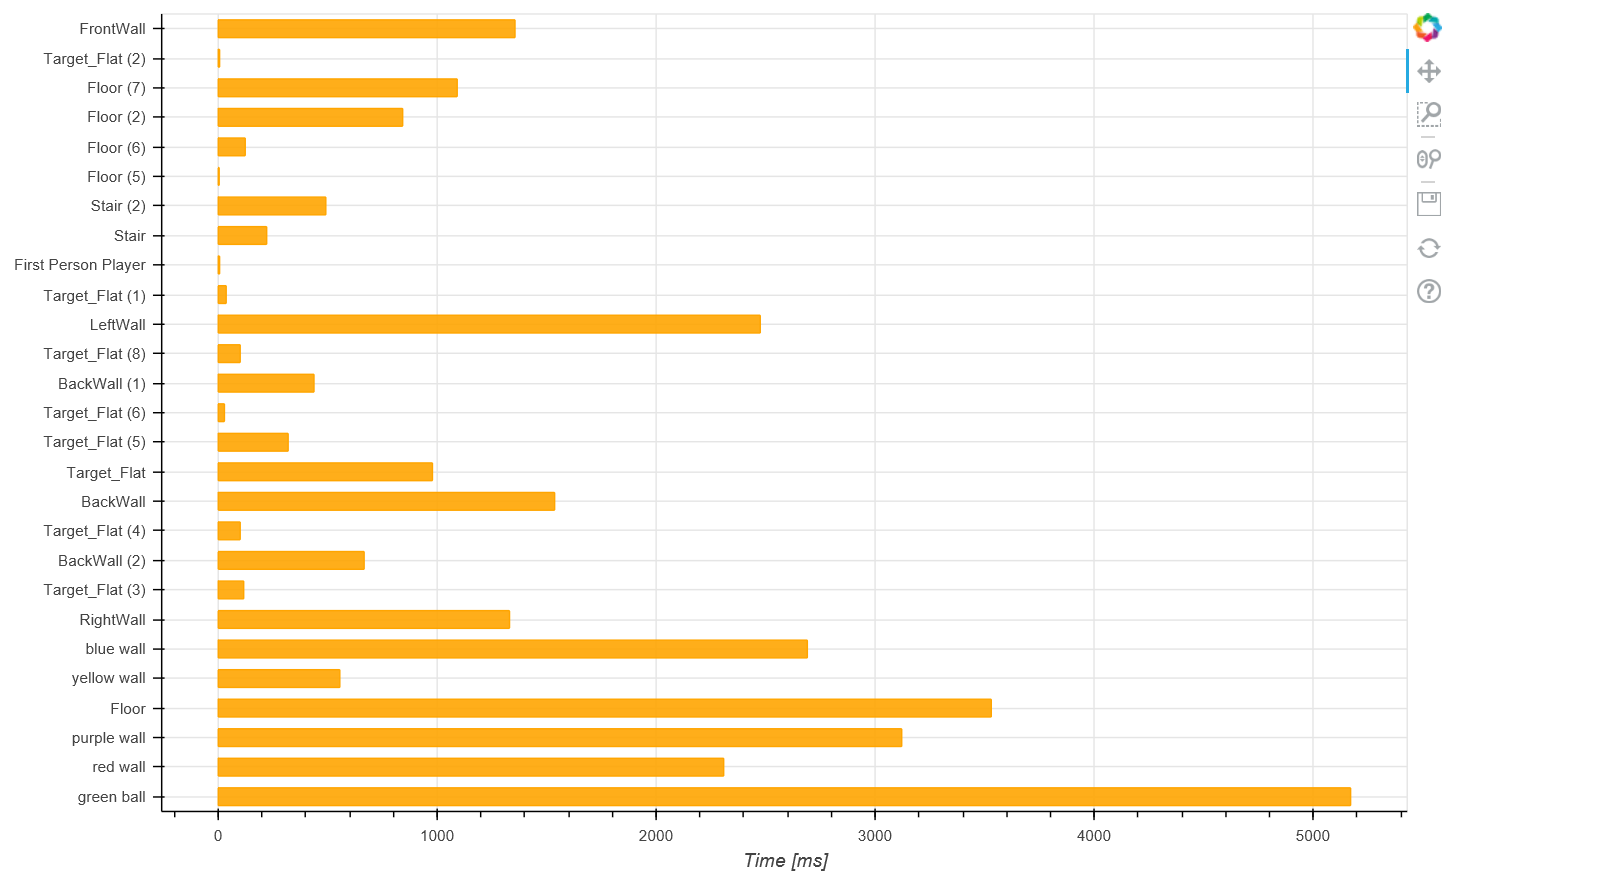
\includegraphics[keepaspectratio,scale=0.3]{GraphStuff.png}
  \caption{Visualization of recorded data}
  \label{fig:graphvisualization}
\end{figure}
\noindent Using a bar chart makes it easy to see what objects the player was looking the most/least. And dependent of what the user wants to study this could be a good way of visualizing the data.
Of course, bokeh is not the only way to visualize the data. For instance, another resource that could be used is the python library matplotlib \cite{matplotlib}.
\newpage
\section{What we would have wanted to add}
\begin{itemize}
\item \textbf{Cross scene data gathering}\\
The package would have supported several scenes and the loading in between them if we had the time.
\item \textbf{Folder structure for CSV files}\\
At the moment all CSV files end up in the same folder which makes it rather time consuming to find the specific file you are looking for.\\
\texttt{'SightTracker/SceneName/DateAndTime/CSVFiles/'} would have been easier to browse.
\end{itemize}
\newpage
\begin{thebibliography}{9}
\bibitem{unitykeycode}
Unity Keycode,
\texttt{https://docs.unity3d.com/ScriptReference/KeyCode.html}
\bibitem{bokeh}
bokeh, 
\texttt{https://docs.bokeh.org/en/latest/index.html}
\bibitem{matplotlib}
matplotlib,
\texttt{https://matplotlib.org/}

\end{thebibliography}
\end{document}